\documentclass[10pt, titlepage, oneside, a4paper]{article}
\usepackage[T1]{fontenc}
%\usepackage[swedish]{babel}
\usepackage{amssymb, graphicx, fancyheadings}
\usepackage{url}
\usepackage[utf8]{inputenc}
\addtolength{\textheight}{20mm}
\addtolength{\voffset}{-5mm}
\renewcommand{\sectionmark}[1]{\markleft{#1}}

\usepackage{lscape}
\usepackage{titlesec}

\newcommand{\scite}[1]{\textsuperscript{\cite{#1}}}
	
\newcounter{appendixpage}

\newenvironment{appendices}{
	\setcounter{appendixpage}{\arabic{page}}
	\stepcounter{appendixpage}
}{
}

\newcommand{\appitem}[2]{
	\stepcounter{section}
	\addtocontents{toc}{\protect\contentsline{section}{\numberline{
	\Alph{section}}#1}{\arabic{appendixpage}}}
	\addtocounter{appendixpage}{#2}
}

\newcommand{\appsubitem}[2]{
	\stepcounter{subsection}
	\addtocontents{toc}{\protect\contentsline{subsection}{\numberline{
	\Alph{section}.\arabic{subsection}}#1}{\arabic{appendixpage}}}
	\addtocounter{appendixpage}{#2}
}

\def\inst{Datavetenskap}
\def\typeofdoc{Report}
\def\course{Operating Systems}
\def\pretitle{Assignment 3}
\def\title{Linux I/O Scheduling}
\def\name{Mikael Karlsson}
\def\email{c12mkn@cs.umu.se}
\def\graders{Ahmed Aley, Jan Erik Moström}


\begin{document}
	\begin{titlepage}
		\thispagestyle{empty}
		\begin{large}
			\begin{tabular}{@{}p{\textwidth}@{}}
				\textbf{Umeå university \hfill \today} \\
				\textbf{\typeofdoc} \\
			\end{tabular}
		\end{large}
		\vspace{10mm}
		\begin{center}
			\LARGE{\pretitle} \\
			\huge{\textbf{\course}}\\
			\vspace{10mm}
			\LARGE{\title} \\
			\vspace{15mm}
			\begin{large}
				\begin{tabular}{ll}
					\textbf{Name} & \name \\
					\textbf{E-mail} & \texttt{\email} \\
					
				\end{tabular}
			\end{large}
			\vspace{15mm} 
			\vfill
			\large{\textbf{Graders}}\\
			\mbox{\large{\graders}}
		\end{center}
	\end{titlepage}


	\lfoot{\footnotesize{\name \\ \email}}
	\rfoot{\footnotesize{\today}}
	\lhead{\sc\footnotesize\title}
	\rhead{\nouppercase{\sc\footnotesize\leftmark}}
	\pagestyle{fancy}
	\renewcommand{\headrulewidth}{0.2pt}
	\renewcommand{\footrulewidth}{0.2pt}

	\pagenumbering{roman}

	\pagenumbering{arabic}
	\setlength{\parindent}{0pt}
	\setlength{\parskip}{10pt}

    \section{Introduction}
        As part of the operating systems course given at Umeå University (fall of 2016), students were tasked with testing and comparing three different I/O schedulers for the Linux Kernel.
        
    \section{Method}
        To compare the different I/O schedulers of Linux, one could think of a number of different tests. Variables may include: what performance metric we are looking at (CPU load, write speed, read speed, latency), what kind of action we will perform (sequential or parallel read/writes, buffered or unbuffered I/O), underlying storage device (mechanical HDDs, SSDs, memory cards) and so on. 
        
        For this assignment, it was decided upon to conduct tests using both sequential and parallel writes on a SD memory card, using buffered I/O and monitoring write speeds. This was decided upon for a number of reasons. Raspberry Pis were readily available as development tools on this course, which natively uses SD cards. Buffered I/O was decided upon as this represents the typical use case scenario when it comes to SD cards. The choice of performance metric ended up being write speeds, as this is both a very sought after property as well as easily comparable. The reason behind choosing writes over reads was that SD card write speeds are commonly lower than read speeds. It seemed more fitting to choose the most contested operation for a benchmark.
        
        The three different schedulers selected for use in the test are cfq, noop, and deadline. These are the most commonly used I/O schedulers and are included in the Linux kernel.
        
        The actual test consists of three different parts, each utilizing a small program written in C which simply writes from memory to a number of files, using a set number of threads. The three tests were designed to benchmark the different I/O schedulers in some different circumstances, writing a large file using a single thread (sequential write), writing a few moderately sized files using a few threads and writing a large number of small files using a large number of thread (parallel writes). All three tests are listed below, the results of each test is documented in the \ref{results} section.
        
        \begin{itemize}
            \item Writing 1 1 GB file using 1 thread. 
            \item Writing 5 100 MB files using 5 threads.
            \item Writing 400 1 MB files using 100 threads.
        \end{itemize}
        
        All tests were run on a Raspberry Pi 3 Model B, running release Jessie of Raspbian with Linux kernel version 4.4.

    \section{Implementation}
       
        The repository for the assignment may be viewed locally at
        
        \texttt{/home/c12/c12mkn/edu/5DV171/assignments/3} 
        
        or as a remote git repository at
        
        \url{https://github.com/currybullen/opsys_assignment_3}
        
        Also, the C code written for the assignment may be found as an appendix to this report.
    
        The test to compare the different I/O schedulers focuses on write speed and was written in C. \texttt{par\_write} (source code may be found under \texttt{src/} as well as at the end of this report) will take 5 arguments, in this particular order: \emph{number of files, file size, number of threads, destination directory} \emph{and buffer size}. Upon running \texttt{par\_write} it will immediately start writing zeroes (reading from \texttt{/dev/zero} to the specified number of files in the specified directory, using the specified number of threads and buffer size. A thread will stop writing to a file once the size of that file has reached the specified size.
        
    \section{Usage}
 
        To compile the source of \texttt{par\_write} simply run \texttt{make} at the root of the git repository. This will generate a runnable object under \texttt{target}. The test may be run directly using this object, with arguments specified in the previous section. However, it is recommended to make use of the shell script that is described in this section instead.
        
        A tool that exists at the root of the git repository, \texttt{par\_writes.sh}, will use the \texttt{par\_writes} C program to run a set of tests. To configure the parameters of the test, the file \texttt{settings.cfg} (also found at the repository root) should be edited. The values listed in \texttt{settings.cfg} are listed below, some are required to be changed, while the rest have a starting value and may optionally be altered.
        
        Required:
        
        \begin{itemize}
            \item \texttt{DEVICE} should be set to the name of the device that tests are being run against. E.g. sda, sdb.
            \item \texttt{NUM\_FILES} will set the number of files to be generated.
            \item \texttt{SIZE} will set size of each file to be generated, in bytes.
            \item \texttt{NUM\_THREADS} sets the number of threads to be used.
        \end{itemize}
        
        Optional:
        
        \begin{itemize}
            \item \texttt{BUF\_SIZE} can be used to change the size of the buffer for the writes. The size is specified in bytes.
            \item \texttt{OUTPUT\_DIR} points to the directory in which the written files will be generated. This SHOULD point to a directory with no important data in, as the script will delete any data within it when it finishes.
            \item \texttt{RESULTS\_DIR} points to the directory where the results of a test run will be put.
        \end{itemize}
        
        Once the values in \texttt{settings.cfg} have been set, it is time to choose a scheduler to test. To change the I/O scheduler for the device that is being tested, make sure that that device has been set in \texttt{settings.cfg} and then run \texttt{set\_scheduler.sh <scheduler>} (note that this script has to be run as root). To double check that the wished scheduler is in use, run \texttt{get\_scheduler.sh}.
        
        To finally run the tests, use \texttt{par\_writes.sh <NUM\_TESTS>} where the argument \texttt{NUM\_TESTS} will decide how many times the test is run. The script will echo a short message every time a test has finished. The results of the tests may then be viewed in the results directory, where one file is generated containing the time for each individual test to finish, and anoher file (suffixed with \texttt{\_avg}) containing the average time for such a test to finish.
        
        \section{Results} \label{results}
        
        \begin{figure}
            \centering
            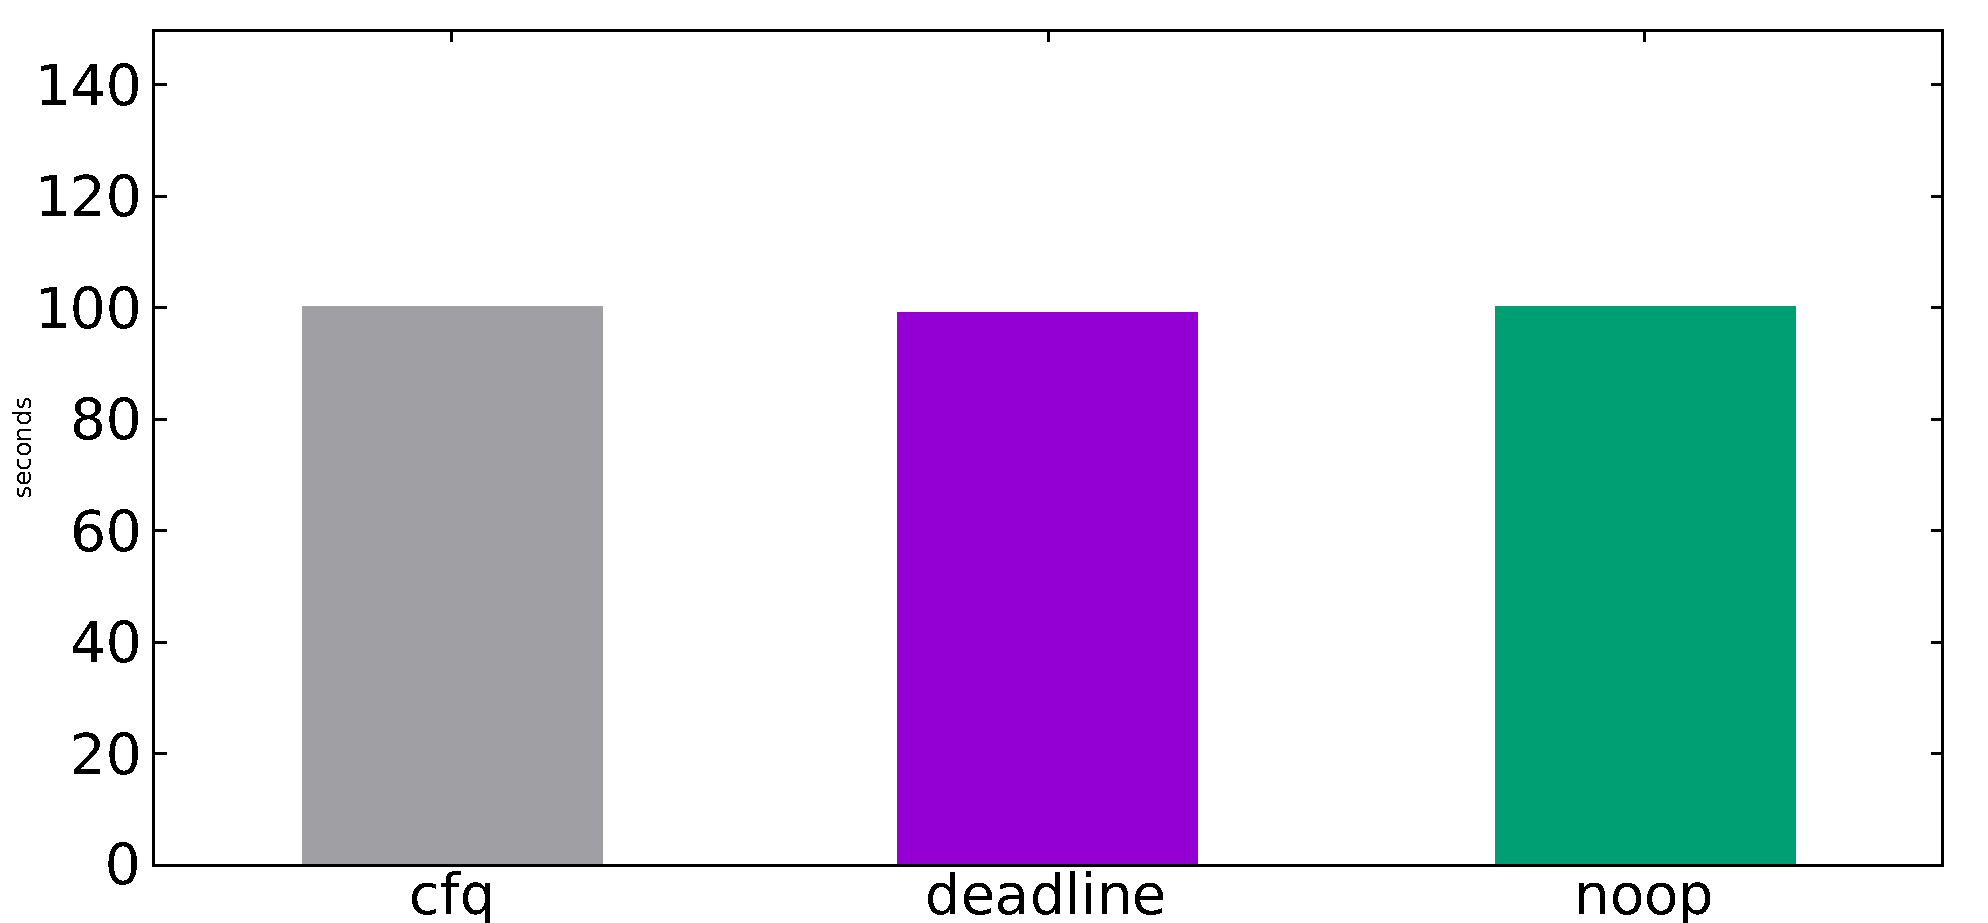
\includegraphics[width=1.0\textwidth]{1f_1gb_1t.pdf}
            \caption{Writing 1 file of size 1 GB using one thread.}
            \label{fig:1f_1gb_1t}
        \end{figure}
        
        \begin{figure}
            \centering
            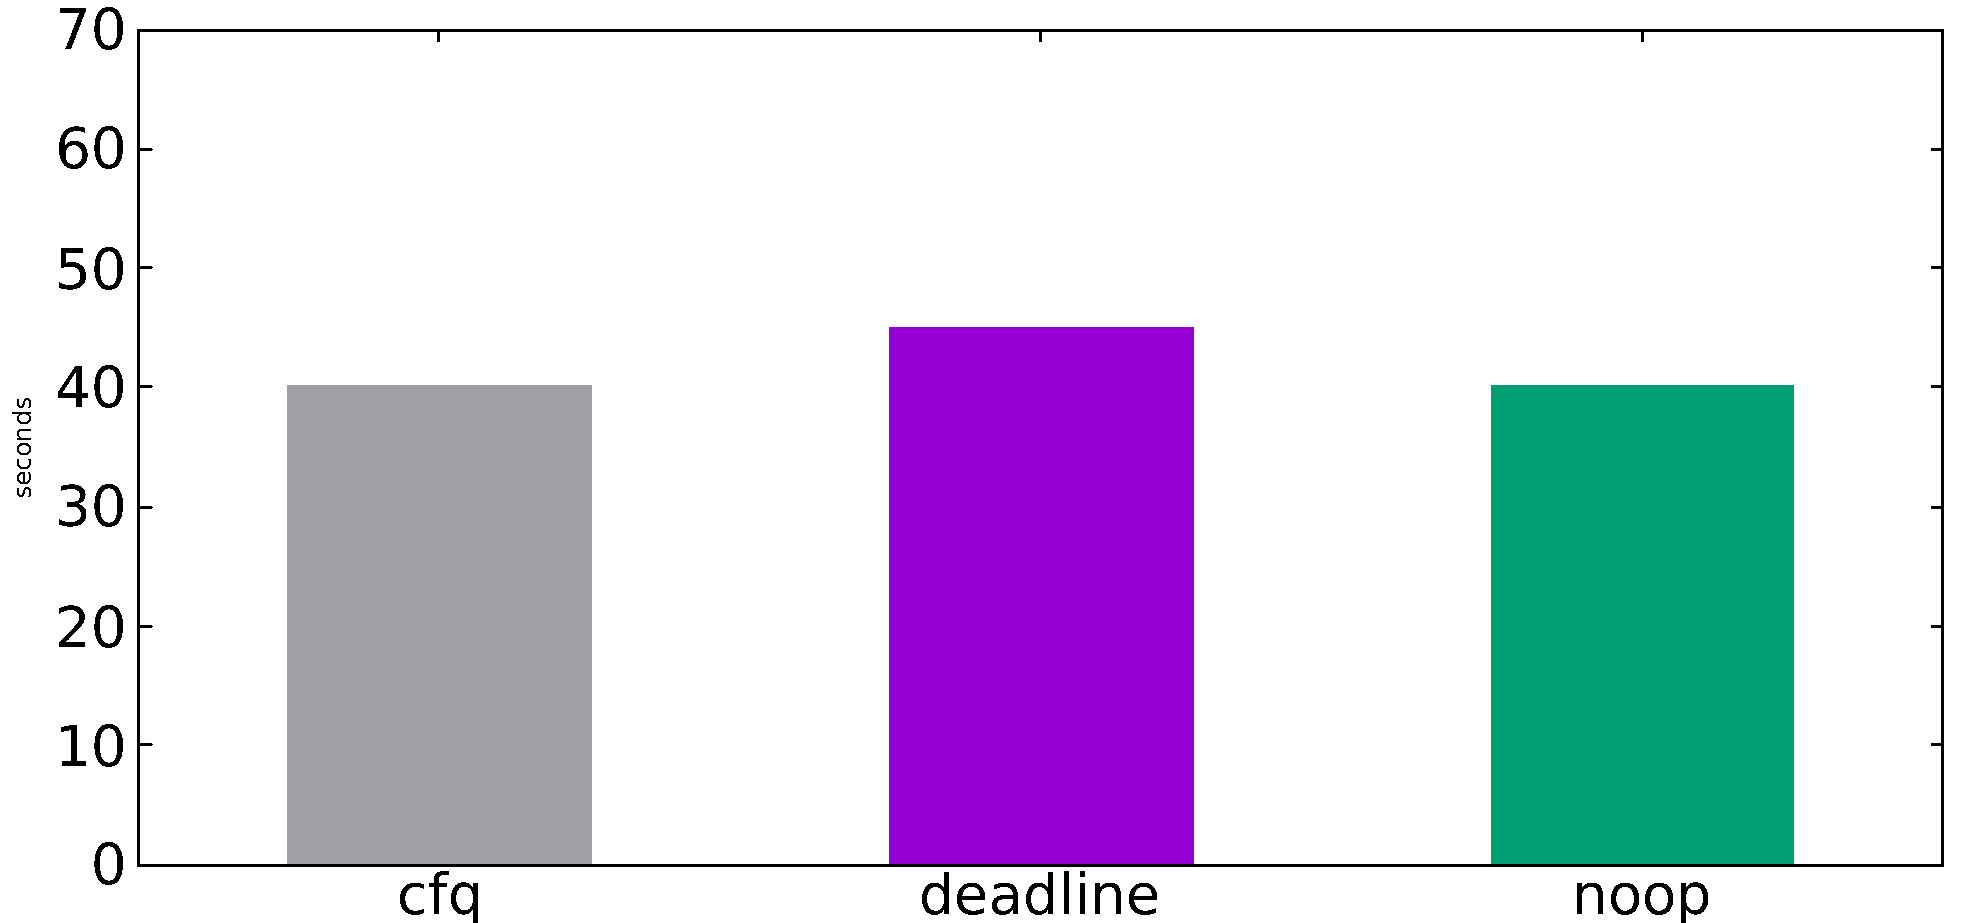
\includegraphics[width=1.0\textwidth]{5f_100mb_5t.pdf}
            \caption{Writing 5 files of size 100 MB using 5 threads.}
            \label{fig:5f_100mb_5t}
        \end{figure}
        
        \begin{figure}
            \centering
            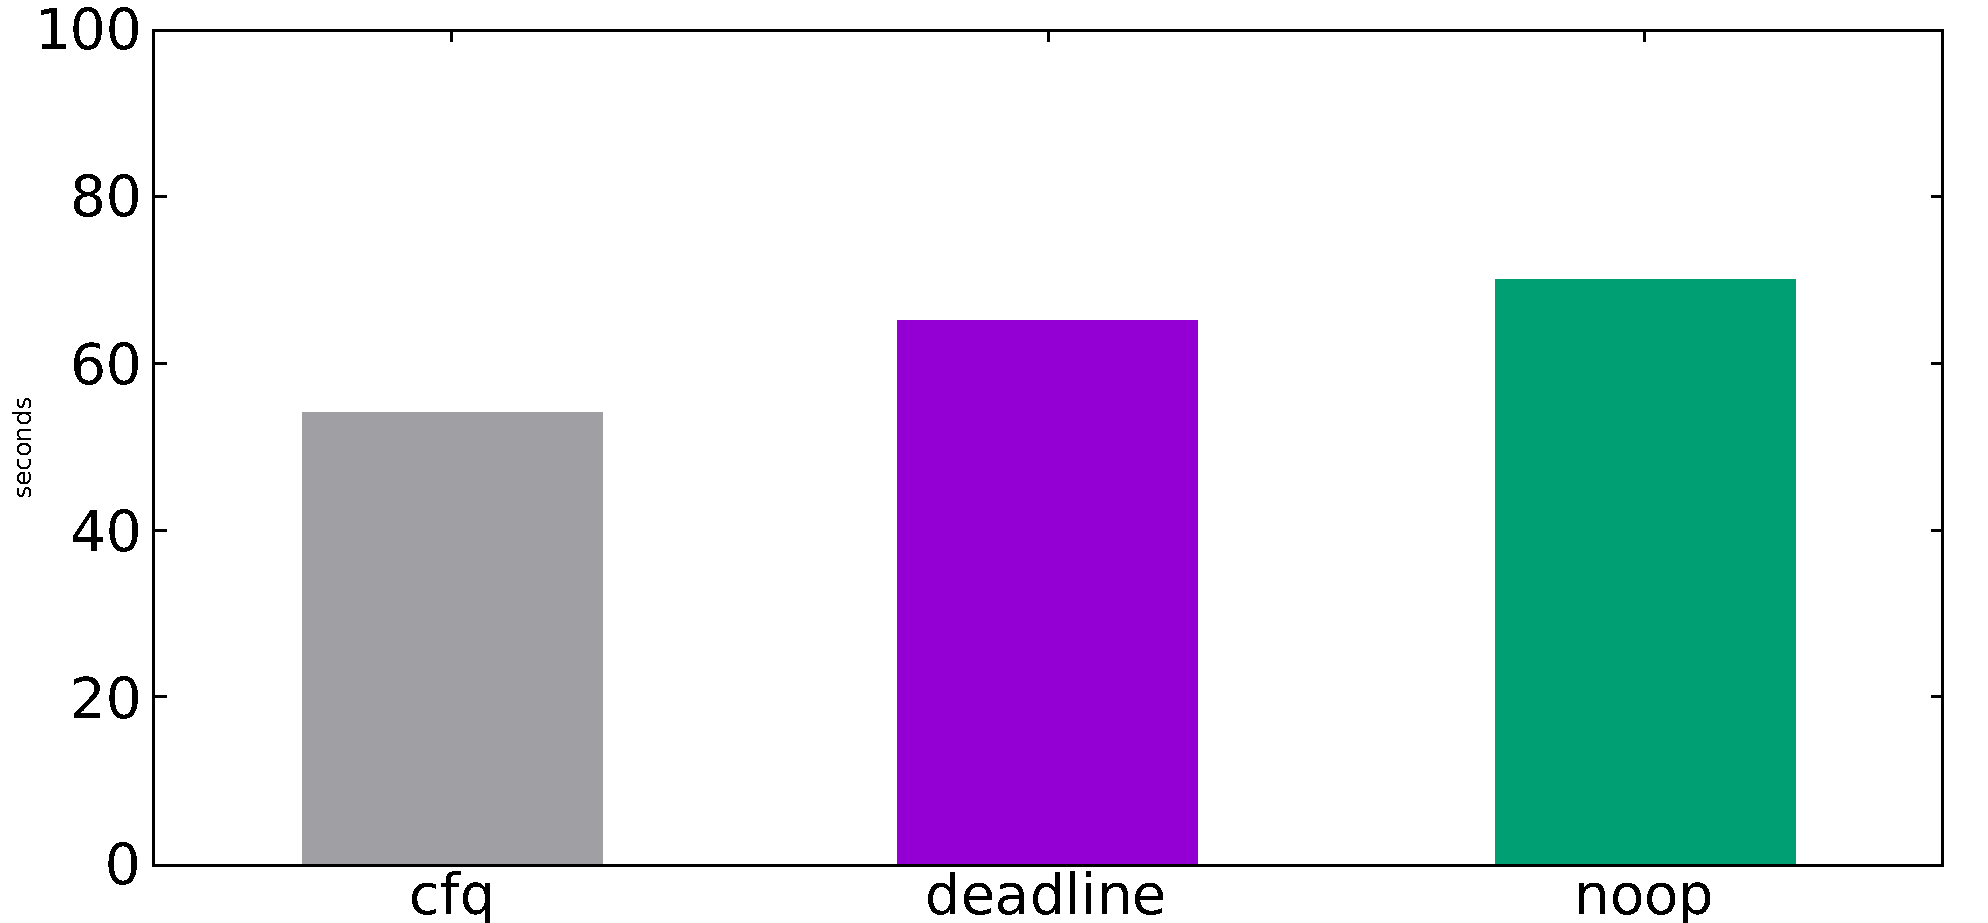
\includegraphics[width=1.0\textwidth]{400f_1mb_100t.pdf}
            \caption{Writing 400 files of size 1 MB using 100 threads.}
            \label{fig:400f_1mb_100t}
        \end{figure}
        

        Figures \ref{fig:1f_1gb_1t}, \ref{fig:5f_100mb_5t} and \ref{fig:400f_1mb_100t} show the results of the tests that were run. Each test was run 10 times, recording the average value for each test.
        
        Looking at \ref{fig:1f_1gb_1t} we see that when writing a large file of 1 GB in size, using only one single thread, there is marginal difference in performance between the different schedulers. On average, the cfq and noop schedulers needed 100 seconds to complete the operation, while the deadline scheduler needed 99 seconds.
        
        \ref{fig:5f_100mb_5t} shows some notable differences when writing 5 moderately sized files using 1 thread per file. The noop and cfq schedulers were the quickest, both needing 45 seconds to complete the operation. The deadline scheduler needed an additional 5 seconds, coming in at 50 seconds total.
        
        When writing 400 files, each 1 MB in size, using 100 threads, \ref{fig:400f_1mb_100t} shows that cfq performed the best, only requiring 54 seconds to finish. The deadline operator finished in 65 seconds, and the noop was the slowest at 70 seconds.
        
        \section{Discussion}
        
        Looking at the test result in \ref{fig:1f_1g_1t} we can conclude that the write speed in a non-parallel application is not severely affected by the choice of scheduler. This makes sense, as there is no I/O operation competition between different processes. The cfq scheduler will only manage a single queue, the I/O queue for the sole running process. This is identical to the noop scheduler which at all times handles only a single FIFO I/O queue. What about the deadline scheduler? If the process manages to queue up enough write requests, to the point where some requests expire beyond their given deadline, some rearrangement of the I/O queue will take place. It is not clear from the test result if any such rearrangement is taking place, however, it is safe to say that if it is, it is not adversely affecting the performance in this case.
        
        In the case of writing 5 files of size 100 MB using 5 threads (\ref{fig:5f_100mb_5t}) deadline is somewhat slower to finish than cfq and noop. How is this? One reason that noop finishes quicker than deadline could be that deadlide, unlike noop, introduces some CPU overhead due to the need of re-arranging the I/O queue. But cfq also re-arranges its I/O queue, should it not be slower then as well? Perhaps, but if anything is to be concluded from the test results, it seems like the CPU overhead that cfq introduces does not impact the total write time as severely as deadline does.
        
        If the assumption that the deadline scheduler imposes a performance loss (in the very specific case of the tests performed in this assignment), this would also explain the performance difference found in the third test of writing 400 1 MB files using 100 threads (\ref{fig:400f_1mb_100t}). The writes carried out using the deadline scheduler were considerably slower than those of the cfq scheduler. During this test, the noop scheduler was the slowest of the bunch. This might be because of the fact that when using a noop scheduler with a large number of threads, the I/O queue make take a very heterogeneous form. The topmost 10 operations might all belong to 10 different processes, imposing a performance loss that might not have been seen had they all belonged to the very same process.
        
            \subsection{Improving the schedulers}
            
            It is difficult as a layman to propose any changes to the three schedulers that are discussed in this report. To me it seems they all have different advantages and disadvantages and are all suited for different situations. A possible improvement to I/O scheduling in general might be to introduce some device that will address the problem of selecting a scheduler intelligently. Such a system would determine what I/O scheduler would be most appropriate given the current situation and change it on the fly. I am however uncertain if such functionality should reside within the kernel or should be implemented as some sort of userspace feedback loop.
        
        \pagebreak
        
        \begin{appendices}
        \section*{Appendix A}
        \scriptsize
        \begin{verbatim}
#include <stdio.h>
#include <stdlib.h>
#include <pthread.h>
#include <time.h>
#include <fcntl.h>
#include <unistd.h>

int NUM_FILES;
int SIZE;
int NUM_THREADS;
char *DESTINATION_DIR;
int BUF_SIZE;

int COUNTER;
pthread_mutex_t LOCK;

void *perform_writes(void *args);
void perform_write(char *path);

int main(int argc, char *argv[]) {
    NUM_FILES = strtol(argv[1], NULL, 0);
    SIZE = strtol(argv[2], NULL, 0);
    NUM_THREADS = strtol(argv[3], NULL, 0);
    DESTINATION_DIR = argv[4];
    BUF_SIZE = strtol(argv[5], NULL, 0);

    pthread_t tid[NUM_THREADS];
    for (int i = 0; i < NUM_THREADS; i++) {
        pthread_create(&(tid[i]), NULL, &perform_writes, NULL);
    }

    for (int i = 0; i < NUM_THREADS; i++) {
        pthread_join(tid[i], NULL);
    }
}

void *perform_writes(void *args) {
    while (1) {
        int file_num;
        char path[100];

        pthread_mutex_lock(&LOCK);
        file_num = COUNTER++;
        pthread_mutex_unlock(&LOCK);

        if (file_num >= NUM_FILES)
            pthread_exit(NULL);

        sprintf(path, "%s/%d", DESTINATION_DIR, file_num);
        perform_write(path);
    }
}

void perform_write(char *path) {
    clock_t start, end;
    int src, dst;
    char buf[BUF_SIZE];
    int remaining = SIZE;
    int read_size;

    start = clock();
    src = open("/dev/zero", O_RDONLY);
    dst = open(path, O_WRONLY | O_CREAT, 0644);
    while (remaining > 0) {
        read_size = (remaining < BUF_SIZE) ? remaining: BUF_SIZE;
        read(src, buf, read_size);
        write(dst, buf, read_size);
        remaining -= read_size;
    }

    close(src);
    close(dst);
    end = clock();
    printf("%f\n", (double) (end - start));
}            
        \end{verbatim}
        \normalsize
        \end{appendices}
\end{document}
